\begin{pastexam}[label={px:gk3-106-ds-01}]{高考三級資訊處理 106 年 第一題}
（申論；20 分）

給定二元樹（binary tree）如下圖，樹高為 4 且共有 7 個節點。
\begin{center}
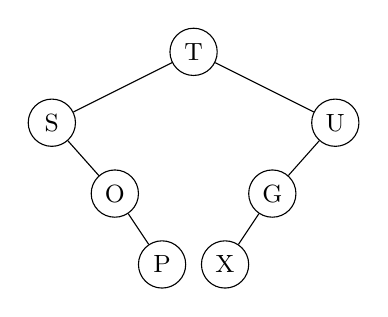
\begin{tikzpicture}[v/.style={circle,draw,minimum size=6mm,inner sep=0pt,font=\small},
    level distance=9mm, level 1/.style={sibling distance=36mm},
    level 2/.style={sibling distance=16mm}, level 3/.style={sibling distance=12mm}]
\node[v] {T}
  child {node[v] {S} child[missing] {} child {node[v] {O} child[missing] {} child {node[v] {P}}}}
  child {node[v] {U} child {node[v] {G} child {node[v] {X}} child[missing] {}} child[missing] {}};
\end{tikzpicture}
\end{center}
\begin{itemize}[leftmargin=2.2em]
\item[㈠] 請寫出該樹之後序遍歷（postorder traversal）結果。（5 分）
\item[㈡] 若以陣列 A[1..15]實作該二元樹，請列舉陣列 A[1..15]的內容。（5 分）
\item[㈢] 若要將數值 x 設為或取代 A[i]（任一 $1 \le i \le 7$）所代表的節點之右子節點（right child node）的
內容，令 x 會被放入陣列中 A[j]的位置。請以 j、i 表示，寫出 j 位置之公式。（5 分）
\item[㈣] 若要在原始的二元樹中加入一些節點使其成為完整二元樹（complete binary tree）及完滿二元樹（full
binary tree），請問最少各需加入幾個新節點？（5 分）
\end{itemize}
\end{pastexam}

\begin{pastsoln}
答案：㈠ P O S X G U T；㈡ 見下表；㈢ $j = 2i + 1$；㈣ 完整二元樹至少加 $5$ 個，完滿二元樹至少加
$8$ 個。

先讀圖：T 的左子節點 S、右子節點 U；S 只有右子節點 O，O 只有右子節點 P；U 只有左子節點 G，G 只有
左子節點 X。 題目說「樹高為 4」，是以節點數計的高度（根在第 1 層，資結書第~7.1~節的約定）。

\textbf{㈠} 後序（左、右、根）：T 的左子樹 S 沒有左子樹，先做右子樹 O：O 的右子樹 P，再 O；然後 S。
右子樹 U：先 G 的子樹 X、G，再 U。 最後 T。 答案 \textbf{P O S X G U T}。

\textbf{㈡} 用陣列存二元樹（資結書第~7.2~節）：根放 $A[1]$，$A[i]$ 的左子節點在 $A[2i]$、右子節點在
$A[2i + 1]$。 逐一定位：
T $= A[1]$；S $= A[2]$、U $= A[3]$（T 的左、右）；O $= A[2 \cdot 2 + 1] = A[5]$；
G $= A[2 \cdot 3] = A[6]$；P $= A[2 \cdot 5 + 1] = A[11]$；X $= A[2 \cdot 6] = A[12]$。 其餘的格子
空著（下表以 -- 表示）：
\begin{center}
\small
\setlength{\tabcolsep}{4pt}
\begin{tabular}{c*{15}{c}}
\toprule
$i$ & 1 & 2 & 3 & 4 & 5 & 6 & 7 & 8 & 9 & 10 & 11 & 12 & 13 & 14 & 15 \\
\midrule
$A[i]$ & T & S & U & -- & O & G & -- & -- & -- & -- & P & X & -- & -- & -- \\
\bottomrule
\end{tabular}
\end{center}
高度 $4$ 的二元樹最多 $2^4 - 1 = 15$ 個節點，所以 $A[1..15]$ 剛好夠用；$7$ 個節點卻用到 15 格，這就
是歪斜的樹用陣列存的浪費。

\textbf{㈢} $A[i]$ 的右子節點在 $\mathbf{j = 2i + 1}$。 理由：第 $k$ 層（根是第 1 層）的節點依序放在
$A[2^{k-1} .. 2^k - 1]$。 $A[i]$ 若是第 $k$ 層從左數來第 $t$ 個（$i = 2^{k-1} + t - 1$），它左邊同層有
$t - 1$ 個位置，每個位置在下一層占兩格，所以它的左子節點是第 $k + 1$ 層的第 $2t - 1$ 個，位置
$2^k + 2t - 2 = 2i$，右子節點緊接著在 $2i + 1$。 題目限定 $1 \le i \le 7$，是為了讓 $2i + 1 \le 15$
還在陣列範圍內。 例：$i = 5$（O）時 $j = 11$，正是 P 的位置。

\textbf{㈣} 名詞依資結書第~7.1~節：\textbf{完整二元樹}（complete）是除了最後一層之外每層都滿、最後一層
的節點都靠左；\textbf{完滿二元樹}（full，有的書叫滿二元樹，也就是 perfect）是每一層都滿，高度 $h$ 時
恰有 $2^h - 1$ 個節點。
\begin{itemize}
\item 完整二元樹：$n$ 個節點的完整二元樹用陣列存時正好占 $A[1..n]$、中間沒有空格。 原樹最右邊的節點
X 在 $A[12]$，而只加節點不能把 X 移走，所以結果至少要占滿 $A[1..12]$；目前 $1$--$12$ 裡空著的是
$A[4]$、$A[7]$、$A[8]$、$A[9]$、$A[10]$，加這 $\mathbf{5}$ 個（分別是 S 的左子節點、U 的右子節點、
新的 $A[4]$ 的兩個子節點、O 的左子節點）就成為 $12$ 個節點的完整二元樹。 少於 $5$ 個做不到，因為
這 $5$ 格都在 X 之前，空著任何一格就不是完整二元樹。
\item 完滿二元樹：原樹高度已經是 $4$，加節點後高度至少 $4$，完滿時至少 $2^4 - 1 = 15$ 個節點，要加
$15 - 7 = \mathbf{8}$ 個，也就是把 $A[1..15]$ 的 $8$ 個空格全部填滿。
\end{itemize}
附帶一提：有些書（多數英文教科書）的 full binary tree 指「每個節點的子節點數是 $0$ 或 $2$」（資結書
叫嚴格二元樹）。 照那個定義，只要替只有一個子節點的 S、O、U、G 各補一個子節點，共 $4$ 個。 本題把
complete 和 full 並列，又給了 $A[1..15]$，採用每層都滿的定義，答 $8$。
\end{pastsoln}
